\documentclass[11pt]{article}
\usepackage[utf8]{inputenc}
\usepackage[T1]{fontenc}
\usepackage[letterpaper,margin=1in]{geometry}
\usepackage{amsmath,amssymb}
\usepackage{graphicx}
\usepackage{booktabs}
\usepackage{enumitem}
\usepackage{xcolor}
\usepackage{listings}
\usepackage{fancyhdr}
\usepackage{hyperref}

\hypersetup{colorlinks=true, linkcolor=blue, urlcolor=blue}

\pagestyle{fancy}
\fancyhf{}
\fancyhead[R]{\small\itshape SEL5917 --- Estimation Theory \ $\vert$\ Exercise: Recursive LS for 2D GNSS Positioning}
\fancyfoot[C]{\thepage}
\renewcommand{\headrulewidth}{0.3pt}

\lstdefinestyle{matlab}{
  backgroundcolor=\color{gray!8},
  basicstyle=\ttfamily\small,
  breaklines=true,
  frame=single,
  framerule=0pt,
  columns=fullflexible,
  keepspaces=true,
  xleftmargin=4pt, xrightmargin=4pt,
  aboveskip=8pt, belowskip=8pt
}

\newcommand{\true}{\text{true}}

\title{\vspace{-1.5em}\textcolor{blue!40!black}{\large SEL5917 --- Estimation, Identification and Stochastic Filtering}\\[0.4em]
\textbf{Exercise: Recursive Least Squares for 2D GNSS Positioning}}
\author{}
\date{}

\begin{document}
\maketitle
\thispagestyle{fancy}
\vspace{-2.5em}

\section{Scenario}

A receiving antenna is located at an unknown fixed position $\theta = (x_a, y_a)$ in a local 2D plane
(units: km). Three GNSS satellites at known positions $S_k = (x_k, y_k)$, $k = 1,2,3$, broadcast ranging
signals. The antenna's receiver measures the pseudorange (distance) to each satellite, one at a time, as
the signals arrive in sequence:
\begin{equation}
  \rho_k = \|\theta - S_k\| + \varepsilon_k, \qquad \varepsilon_k \sim \mathcal{N}(0,\sigma^2), \qquad
  \sigma = 0.05\ \text{km} \ (\approx 50\ \text{m}).
\end{equation}

The satellite positions are given in Table~\ref{tab:sats}, together with a plot of the geometry
(satellites, the true --- unknown --- antenna position, and a nominal starting point $\theta_0$ used
later for linearization), shown in Figure~\ref{fig:geometry}.

\begin{table}[h]
\centering
\caption{Known satellite positions.}
\label{tab:sats}
\begin{tabular}{@{}lcc@{}}
\toprule
Satellite & $x$ (km) & $y$ (km) \\
\midrule
$S_1$ & 20.0  & 5.0  \\
$S_2$ & $-15.0$ & 18.0 \\
$S_3$ & 10.0  & $-20.0$ \\
\bottomrule
\end{tabular}
\end{table}

\begin{figure}[h]
\centering
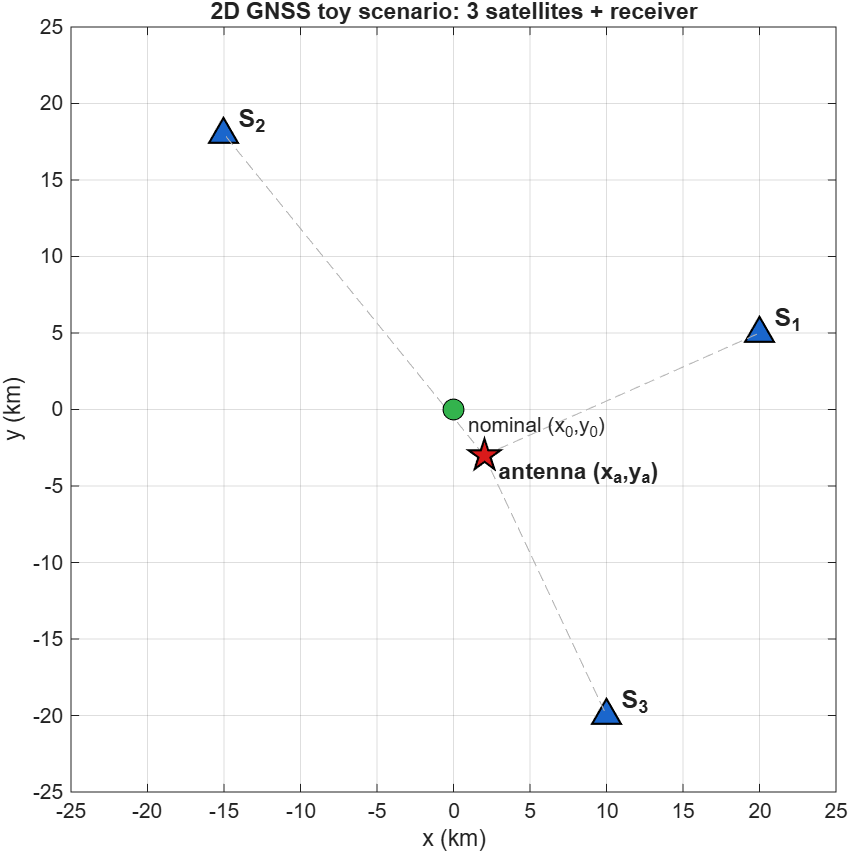
\includegraphics[width=0.55\textwidth]{images/gnss_2d_geometry.png}
\caption{2D GNSS toy scenario: 3 satellites and the receiver.}
\label{fig:geometry}
\end{figure}

The three (simulated) pseudorange measurements, received sequentially as satellites 1, 2 and 3 come into
view, are:
\begin{equation}
  \rho_1 = 19.6708\ \text{km}, \qquad \rho_2 = 27.0619\ \text{km}, \qquad \rho_3 = 18.8371\ \text{km}.
\end{equation}

\section{Task 1 --- Why is this not directly a linear ML problem?}

The lecture derived the recursive Maximum Likelihood estimator for the linear model
$y_k = H_k\theta + \varepsilon_k$. Here, $\rho_k = \|\theta - S_k\| + \varepsilon_k$ is a nonlinear
function of $\theta$.

\begin{enumerate}[leftmargin=2.2em]
\item Write $\rho_k$ explicitly as a function of $x_a$, $y_a$, $x_k$ and $y_k$, and confirm it is
      nonlinear in $\theta = (x_a,y_a)$.
\end{enumerate}

\section{Task 2 --- Linearize around a nominal point}

To recover a linear measurement equation, linearize $\rho_k(\theta)$ with a first-order Taylor expansion
around a nominal / initial-guess position $\theta_0 = (x_0,y_0)$ --- here we take $\theta_0 = (0,0)$,
i.e.\ ``start at the origin'':
\begin{equation}
  \rho_k(\theta) \approx \rho_k(\theta_0) + H_k(\theta - \theta_0), \qquad
  H_k = \left.\frac{\partial \rho_k}{\partial \theta}\right|_{\theta_0}
      = \left[\frac{x_0-x_k}{\rho_{0,k}},\ \frac{y_0-y_k}{\rho_{0,k}}\right],
\end{equation}
where $\rho_{0,k} = \|\theta_0 - S_k\|$ is the (known) nominal range. Defining the linearized measurement
$\Delta\rho_k := \rho_k - \rho_{0,k}$ and the unknown $\Delta\theta := \theta - \theta_0$, this gives
exactly the linear model studied in class:
\begin{equation}
  \Delta\rho_k = H_k\,\Delta\theta + \varepsilon_k, \qquad \varepsilon_k \sim \mathcal{N}(0,R), \qquad R = \sigma^2.
\end{equation}

\begin{enumerate}[leftmargin=2.2em]
\setcounter{enumi}{1}
\item For each $k=1,2,3$, compute $\rho_{0,k}$, $H_k$, and $\Delta\rho_k$, using $\theta_0=(0,0)$ and the
      satellite table above. Fill in Table~\ref{tab:linearized} (values rounded to 4 decimals are given
      for you to check your work).
\end{enumerate}

\begin{table}[h]
\centering
\caption{Linearized measurements.}
\label{tab:linearized}
\begin{tabular}{@{}cccc@{}}
\toprule
$k$ & Pseudorange $\rho_k$ (km) & Nominal range $\rho_{0,k}$ (km) & $\Delta\rho_k = \rho_k - \rho_{0,k}$ (km) \\
\midrule
1 & 19.6708 & 20.6155 & $-0.9447$ \\
2 & 27.0619 & 23.4307 & 3.6311 \\
3 & 18.8371 & 22.3607 & $-3.5236$ \\
\bottomrule
\end{tabular}
\end{table}

\section{Task 3 --- Apply the Recursive ML (RLS) Estimator}

Using the recursive form derived in class,
\begin{align}
  \hat{\Delta\theta}_k &= \hat{\Delta\theta}_{k-1} + K_k\big(\Delta\rho_k - H_k \hat{\Delta\theta}_{k-1}\big), \\
  K_k &= P_k H_k^\top R^{-1} = P_{k-1}H_k^\top\big(R + H_k P_{k-1}H_k^\top\big)^{-1}, \\
  P_k &= [I - K_k H_k]\,P_{k-1},
\end{align}
with a vague (uninformative) prior $\hat{\Delta\theta}_0 = 0$ and $P_0 = 10^6 \cdot I_2$ (no prior
knowledge of the position error):

\begin{enumerate}[leftmargin=2.2em]
\setcounter{enumi}{2}
\item Process the three measurements one at a time, in order $k=1,2,3$. After each step, report
      $\hat{\Delta\theta}_k$ and the estimated antenna position $\hat\theta_k = \theta_0 + \hat{\Delta\theta}_k$.
\item Report the final estimate $\hat\theta = (\hat x_a, \hat y_a)$ after all 3 satellites have been
      processed, and the final covariance $P_3$ (how confident is the estimate in each coordinate?).
\end{enumerate}

\section{Task 4 --- Check against the Batch ML/LS Solution}

Stack the three linearized measurements into $\Delta z = [\Delta\rho_1;\, \Delta\rho_2;\, \Delta\rho_3]$
and $\mathcal{H} = [H_1;\, H_2;\, H_3]$, and compute the batch estimator
\begin{equation}
  \hat{\Delta\theta}^{\text{ML}} = (\mathcal{H}^\top \mathcal{H})^{-1}\mathcal{H}^\top \Delta z.
\end{equation}

\begin{enumerate}[leftmargin=2.2em]
\setcounter{enumi}{4}
\item Verify that the batch solution equals the recursive estimate obtained after processing all 3
      satellites (Task 3). This confirms the equivalence proven in class between the batch and recursive
      ML estimators.
\end{enumerate}

\section{Task 5 --- Discussion (bonus)}

\begin{enumerate}[leftmargin=2.2em]
\setcounter{enumi}{5}
\item With only 2 unknowns $(x_a,y_a)$, 2 satellites in general position already make the linearized
      system exactly determined. Why is a 3rd satellite still useful in practice? Relate your answer to
      the covariance $P_k$ obtained at each step.
\item What happens to the geometry (and to $P_k$) if the 3 satellites are nearly collinear as seen from
      the receiver? (This effect is known in GNSS as poor ``geometric dilution of precision'', GDOP.)
\item Implement Tasks 3--4 in MATLAB (or Python) and confirm your hand computations. Re-run with a
      poorly-placed set of satellites and comment on how $P_k$ changes.
\end{enumerate}

\vspace{0.5em}
\noindent\hrulefill

\vspace{0.3em}
\noindent{\small\itshape Note: the linearization above uses a single nominal point $\theta_0$ for all
three measurements. In a real GNSS receiver this procedure is iterated (Gauss--Newton), re-linearizing
around the latest estimate, and a 4th unknown (receiver clock bias) is included. Both simplifications
were made here so the exercise maps directly onto the linear recursive ML framework covered in class.}

\clearpage
\section*{\textcolor{red!60!black}{Appendix --- Solution Key}}
\noindent{\itshape\textcolor{red!60!black}{(for the instructor --- remove before distributing to students)}}

\subsection*{True (simulated) receiver position}
$\theta_{\true} = (x_a,y_a) = (2.0000,\, -3.0000)$ km --- used only to generate the data, unknown to the
student.

\subsection*{Step-by-step recursive solution}

\begin{table}[h]
\centering
\begin{tabular}{@{}cccc@{}}
\toprule
$k$ & $H_k$ & $\hat\theta_k$ (recursive) [km] & $P_k$ diag [km$^2$] \\
\midrule
1 & $[-0.9701,\ -0.2425]$ & $[0.9165,\ 0.2291]$   & large \\
2 & $[0.6402,\ -0.7682]$  & $[1.7838,\ -3.2401]$  & $\downarrow$ \\
3 & $[-0.4472,\ 0.8944]$  & $[1.7781,\ -3.1364]$  & $[0.0020,\ 0.0021]$ \\
\bottomrule
\end{tabular}
\end{table}

\noindent Final covariance after $k=3$:
$P_3 = \begin{bmatrix} 0.0020 & 0.0009 \\ 0.0009 & 0.0021 \end{bmatrix}$ km$^2$
(std $\approx 45$ m in $x$, $46$ m in $y$).

\subsection*{Batch check}
$\hat\theta_{\text{batch}} = (1.7781,\, -3.1364)$ km --- identical to the recursive result after
$k=3$, as expected.

\subsection*{Reference MATLAB code}
\begin{lstlisting}[style=matlab]
sat = [20 5; -15 18; 10 -20];
xa_true = 2; ya_true = -3; theta0 = [0;0]; sigma = 0.05; R = sigma^2;
N = size(sat,1);
rho0 = vecnorm(theta0' - sat, 2, 2);
H = (theta0' - sat) ./ rho0;
rho_true = sqrt((xa_true-sat(:,1)).^2 + (ya_true-sat(:,2)).^2);
rng(42); rho_meas = rho_true + sigma*randn(N,1);
dz = rho_meas - rho0;

P = 1e6*eye(2); dtheta = zeros(2,1);
for k = 1:N
    Hk = H(k,:);
    K  = P*Hk'/(Hk*P*Hk' + R);
    dtheta = dtheta + K*(dz(k) - Hk*dtheta);
    P = (eye(2)-K*Hk)*P;
    theta_hat = theta0 + dtheta          %#ok<NOPTS>
end
theta_batch = theta0 + (H'*H)\(H'*dz)
\end{lstlisting}

\end{document}
